\chapter{Energy Optimization}
\label{ch:optimization}

\section{Objective Function}

The MILP optimizer minimizes the total daily operating cost over a 24-hour horizon ($T = 96$ steps at $\Delta t = 15$~min):

\begin{equation}
    \min \sum_{t=1}^{T} \left[ C_{\text{grid}}(t) \cdot P_{\text{grid}}(t) \cdot \Delta t + C_{\text{deg}}(t) + \lambda_{\text{peak}} \cdot P_{\text{peak}} \right]
    \label{eq:objective}
\end{equation}

where:
\begin{itemize}[nosep]
    \item $C_{\text{grid}}(t)$ = electricity tariff at time $t$ (1.20~MAD/kWh off-peak, 1.80~MAD/kWh during 18:00--23:00)
    \item $C_{\text{deg}}(t)$ = battery degradation cost (0.15~MAD/kWh discharged)
    \item $\lambda_{\text{peak}}$ = peak demand penalty coefficient
    \item $P_{\text{peak}}$ = maximum grid import over the horizon
\end{itemize}

\section{Constraints}

Subject to:
\begin{enumerate}[nosep]
    \item Energy balance (Equation~\ref{eq:balance}) at every time step
    \item SOC bounds (Equation~\ref{eq:soc_bounds})
    \item Battery power limits (Equations~\ref{eq:ch_limit}--\ref{eq:dis_limit})
    \item No simultaneous charge/discharge (binary variable $z(t)$)
    \item Grid import $\geq 0$
    \item Flexible load scheduling: each load starts at most once within its allowed time window
\end{enumerate}

\section{Flexible Load Scheduling}

For each flexible load $j$, a binary variable $x_j(s) \in \{0, 1\}$ indicates whether load $j$ starts at step $s$. The constraint:

\begin{equation}
    \sum_{s \in S_j} x_j(s) \leq 1
\end{equation}

ensures each load runs at most once. When $x_j(s) = 1$, the load's power is added to the total demand for steps $s$ through $s + d_j - 1$, where $d_j$ is the load's duration in time steps.

The optimizer tends to schedule flexible loads during midday PV surplus periods, reducing grid imports during peak tariff hours.

\section{Solver}

The PuLP library with the CBC solver is used. The 96-step MILP with $\sim$600 variables (including binaries) and $\sim$500 constraints solves in under 1 second per day, well within the requirement.

\section{Comparison: Rule-Based vs MILP}

\subsection{Strategy A --- Rule-Based (Baseline)}

A reactive strategy:
\begin{enumerate}[nosep]
    \item If $P_{\text{PV}} > P_{\text{load}}$: charge battery with surplus
    \item If $P_{\text{PV}} < P_{\text{load}}$: discharge battery if SOC sufficient
    \item Remaining deficit: import from grid
\end{enumerate}

No forecasting, no load shifting, no tariff awareness.

\subsection{Strategy B --- MILP-Optimized}

Uses consumption and PV forecasts to proactively:
\begin{itemize}[nosep]
    \item Reserve battery capacity for evening peak-tariff hours
    \item Schedule flexible loads during PV surplus periods
    \item Minimize peak grid demand
\end{itemize}

\subsection{Fault Tolerance}

If the MILP solver fails (infeasible input due to anomalous data or extreme conditions), the system gracefully falls back to the rule-based strategy. This ensures continuous operation under all conditions, as specified in the design requirements.

\begin{figure}[H]
    \centering
    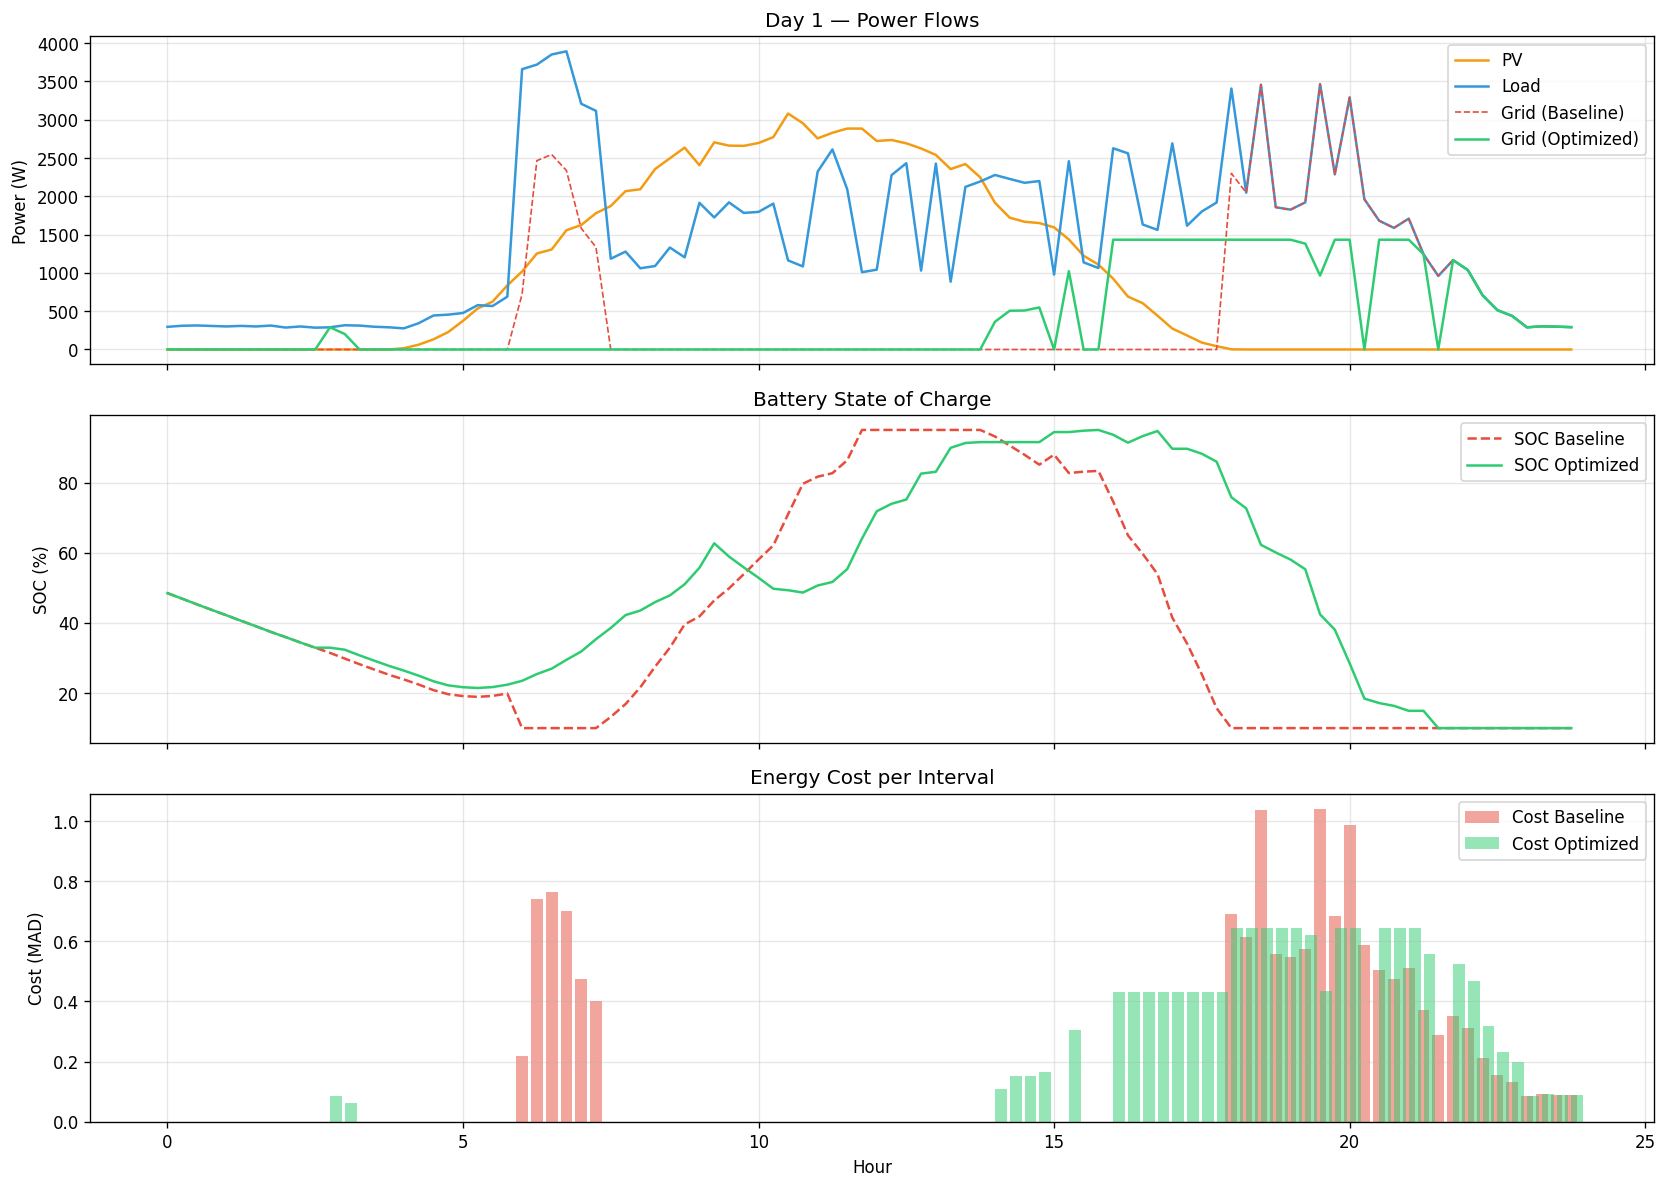
\includegraphics[width=\textwidth]{figures/optimization_day1.png}
    \caption{Day 1 comparison: power flows, battery SOC, and energy cost --- baseline (dashed red) vs optimized (green).}
    \label{fig:opt_day1}
\end{figure}

\begin{figure}[H]
    \centering
    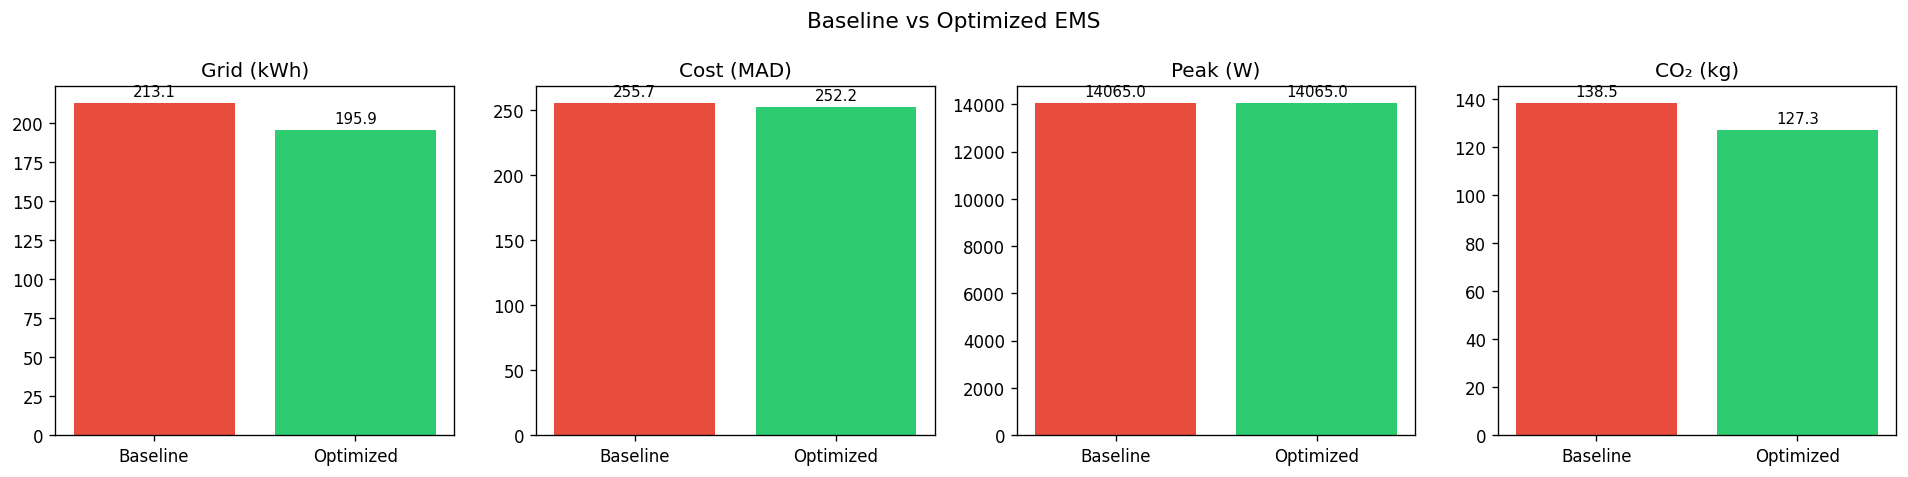
\includegraphics[width=0.85\textwidth]{figures/optimization_bars.png}
    \caption{Baseline vs optimized EMS --- key metrics comparison.}
    \label{fig:opt_bars}
\end{figure}
